\documentclass{article}

\usepackage{neurips_2026}

% Workshop-required footer replacement only (no geometry/font/spacing changes).
\makeatletter
\renewcommand{\@noticestring}{%
  Submitted to the 9th Workshop on Machine Learning and the Physical Sciences (ML4PS 2026). Do not distribute.%
}
\makeatother

\usepackage[utf8]{inputenc}
\usepackage[T1]{fontenc}
\usepackage{hyperref}
\usepackage{url}
\usepackage{booktabs}
\usepackage{amsmath,amssymb}
\usepackage{graphicx}
\usepackage{microtype}

\hypersetup{
  pdfauthor={},
  pdfcreator={},
  pdfproducer={},
  pdftitle={How Representation Curvature Organizes Photometric Decoding in Astronomical Foundation Models},
  pdfsubject={},
  pdfkeywords={}
}

\title{How Representation Curvature Organizes Photometric Decoding in Astronomical Foundation Models}

\author{
  Anonymous Author(s)
}

\begin{document}
\maketitle

\begin{abstract}
Astronomical foundation models are routinely read out with linear probes, yet it remains unclear how scientifically useful information is organized in their representation geometry.
We study a frozen ViT-B galaxy embedding and a photometric $r$-band magnitude target, constructing local quadratic charts on the unit sphere and a split-half sphere-normal mean-curvature statistic $K_H^{\mathrm{cross}}$.
At a frozen chart rank and neighbourhood bandwidth ($d{=}16$, $k{=}2048$, $n{=}512$ anchors), greater curvature energy is associated with worse global linear decoding (controlled Spearman $\rho{\approx}-0.240$ for local OOF $R^2$ and $\rho{\approx}{+}0.227$ for MSE).
The same neighbourhoods exhibit held-out quadratic structure in chart coordinates: an unrestricted quadratic label map improves over a tangent-linear map (median $\Delta_Q{\approx}{+}0.021$), and that gain increases with curvature ($\rho{\approx}{+}0.111$).
The label Hessian aligns with high-energy sphere-normal bending modes, but the associated quadratic family is algebraically full rank: sphere-normal geometry supplies an informative anisotropic prior rather than a low-dimensional constraint.
The association is rank- and bandwidth-conditioned, not claimed to be scale-invariant.
\end{abstract}

\section{Introduction}
\label{sec:intro}

Linear probes are a standard way to ask whether a foundation-model representation contains a scientific observable~\citep{alain2017probes}.
In astronomy this question is now asked of large vision embeddings of galaxies~\citep{duraphe2025platonicuniverse}, against a background hypothesis that foundation models converge toward shared geometric structure~\citep{huh2024platonic}.
Linear decodability, however, need not be uniform across representation space: local extrinsic bending of the activation chart may mark either lost information or information that is organized nonlinearly.

We separate those possibilities at a frozen configuration of one ViT-B~\citep{dosovitskiy2021vit} galaxy embedding.
First we test whether sphere-normal mean-curvature energy co-varies with the error of a \emph{global} linear probe evaluated locally.
Then we test whether the photometric label itself has held-out quadratic structure in the same chart coordinates, whether that structure is more useful in high-curvature neighbourhoods, and whether the fitted label Hessian is oriented along the chart's high-energy bending modes.

\paragraph{Contributions.}
(i)~At frozen rank and bandwidth, reliable sphere-normal curvature is associated with direct global-probe error, not merely an $R^2$ denominator effect.
(ii)~Local photometric labels contain curvature-linked held-out quadratic structure in chart coordinates.
(iii)~Label Hessians align with sphere-normal bending modes, so geometry acts as an informative quadratic prior rather than an algebraically restricted function class.

\section{Method}
\label{sec:method}

\paragraph{Data, model, and target.}
We use a frozen ViT-B embedding of galaxy images (unit-sphere activations) and $n{=}512$ hash-stable anchors with $k{=}2048$ neighbours, aligned throughout by object \texttt{sample\_id}.
The scientific target is an astronomical photometric observable---apparent $r$-band magnitude---not a fundamental physical property and not a spectroscopic DESI label.
A five-fold ridge probe ($\alpha{=}100$) maps embeddings to this magnitude; all probe metrics below are out-of-fold (OOF).
The primary global-decoding outcome is the local OOF coefficient of determination $R_G^2$ of that probe, together with local OOF MSE.
Catalog magnitude as a raw vector is never substituted for either quantity.

\paragraph{Charts and curvature.}
At an anchor $x_0$ we form tangent coordinates $u$ in a nested PCA frame $J$ of dimension $d$ after removing the radial component on the unit sphere, following the local-quadratic charting tradition~\citep{donoho2003hessian}.
A regularized quadratic chart
\[
f(u)=x_0+Ju+\tfrac12 Q(u,u)
\]
is fit with split-half cross-evaluation.
Tangential warp and the forced unit-sphere radial component are removed, leaving a sphere-normal second-fundamental-form tensor $B^S$.
The sphere-normal mean-curvature vector is $H^S=d^{-1}\sum_a B^S_{aa}$; the production statistic is the split-half inner product $K_H^{\mathrm{cross}}=\langle H^{(A)},H^{(B)}\rangle$.
The cross product avoids the positive noise bias of $\|\widehat H\|^2$.
We call this finite-scale \emph{sphere-normal extrinsic bending}, not intrinsic Riemannian curvature of an unknown manifold.
The frozen scientific configuration is $d{=}16$, $k{=}2048$.

\paragraph{Quadratic label models.}
On the same neighbourhoods and outer OOF folds we compare a tangent-linear map $\hat y_L(u)=a_0+a_1^\top u$ with an unrestricted quadratic
$\hat y_{UQ}(u)=a_0+a_1^\top u+\tfrac12 u^\top\Gamma u$
($\Gamma=\Gamma^\top$; $q{=}136$ coefficients at $d{=}16$).
A sphere-normal-constrained map uses $\gamma_{BS}=B_{\mathrm{flat}}^{S\top}c$.
Linear and quadratic blocks are ridge-penalized with nested cross-validation inside each outer training fold, an unpenalized intercept, and a single train-only RMS scale for $u$.
The label Hessian $\Gamma$ describes second-order variation of the photometric target in local chart coordinates.

\paragraph{Inference.}
Controls are $\log$ $k$NN radius, local label variance, and evaluation count.
Primary tests use $B{=}10^4$ rank-space Freedman--Lane permutations and $B{=}2000$ bootstrap intervals; $p{=}0$ is reported as $p<1/(B{+}1)$.
The two primary quadratic hypotheses are Holm-corrected.

\section{Results}
\label{sec:results}

\paragraph{Global linear decoding.}
At the frozen configuration, greater $K_H^{\mathrm{cross}}$ is associated with worse local OOF linear decoding of photometric magnitude, with
$\rho_{\mathrm{ctl}}(K_H^{\mathrm{cross}},R_G^2)\approx-0.240$
and
$\rho_{\mathrm{ctl}}(K_H^{\mathrm{cross}},\mathrm{MSE}_G)\approx{+}0.227$
(Fig.~\ref{fig:global}; $n{=}512$).
The MSE association rules out an $R^2$-denominator explanation: curvature tracks higher squared error, not merely a change in local target variance (controlled $\rho$ with local SST $\approx-0.025$).
The result is conditioned on chart rank and neighbourhood bandwidth (at the same $k$, controlled $R^2$ is $+0.143$ at $d{=}12$ and $-0.233$ at $d{=}20$); we do not claim scale invariance.

\begin{figure}[t]
\centering
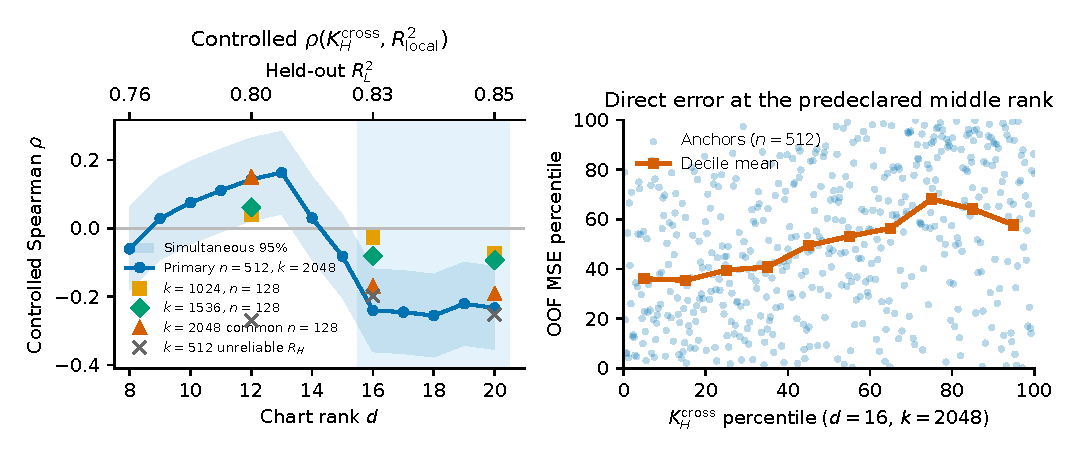
\includegraphics[width=0.90\linewidth]{figures/fig1_global.pdf}
\caption{Confirmatory frozen analysis ($n{=}512$, $k{=}2048$).
Left: controlled $\rho(K_H^{\mathrm{cross}},R_G^2)$ versus chart rank; the scientific configuration is the predeclared middle rank $d{=}16$.
Right: percentile relationship between curvature and local OOF MSE at $d{=}16$.
Scale markers use a smaller $n{=}128$ subset and are not power-matched.}
\label{fig:global}
\end{figure}

\paragraph{Held-out quadratic structure.}
Define $\Delta_Q=\mathrm{MSE}_L-\mathrm{MSE}_{UQ}$.
Median $\Delta_Q\approx{+}0.021$ (bootstrap 95\% CI $[0.0197,0.0216]$); the gain is positive at all $512$ anchors ($p_{\mathrm{MC}}<1/2001$).
Curvature predicts that gain:
$\rho_{\mathrm{ctl}}(K_H^{\mathrm{cross}},\Delta_Q)\approx{+}0.111$ ($p_{\mathrm{MC}}{\approx}0.0075$).
Both primary tests pass Holm correction (Fig.~\ref{fig:quad}a,b).
Local labels therefore exhibit reproducible held-out quadratic structure in chart coordinates, and that structure becomes more predictively useful in neighbourhoods with greater sphere-normal curvature energy.
No causal claim is made.

\begin{figure}[t]
\centering
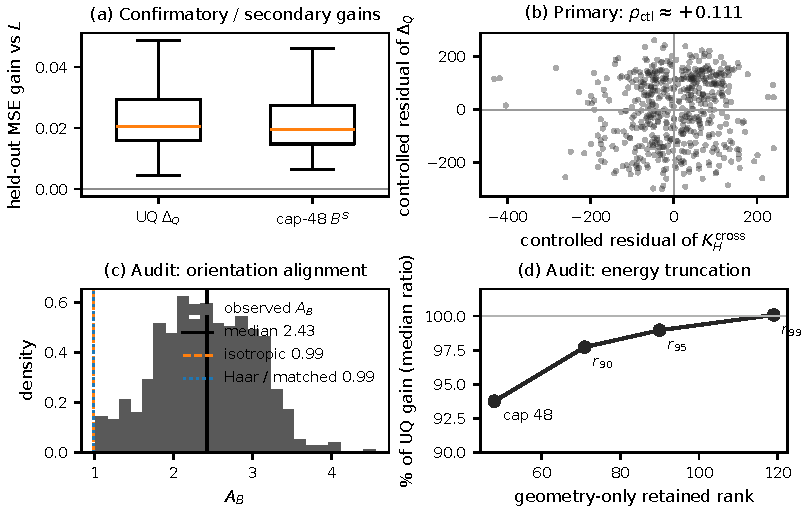
\includegraphics[width=0.90\linewidth]{figures/fig2_quadratic.pdf}
\caption{Quadratic decoding (confirmatory a,b; secondary/audit c,d).
(a)~Held-out MSE gain versus the tangent-linear map $L$.
(b)~Controlled rank residuals of $K_H^{\mathrm{cross}}$ versus $\Delta_Q$.
(c)~Observed Hessian--curvature alignment $A_B$ against isotropic and Haar nulls.
(d)~Median per-anchor fraction of unrestricted quadratic gain retained by geometry-only truncations of $B^S$.}
\label{fig:quad}
\end{figure}

\paragraph{Geometry as an anisotropic prior.}
$B^S_{\mathrm{flat}}$ is algebraically full rank $136$ at every anchor.
Median energy ranks are $r_{90}{=}71$, $r_{95}{=}90$, $r_{99}{=}119$; the original constrained model retained $48$ modes because of a hard cap, not because $48$ modes contain nearly all bending energy.
Full-rank ridge on $c$ is equivalent to unrestricted quadratic regression with the geometry-derived penalty $\gamma^\top(B^{S\top}B^S)^+\gamma$.
Sphere-normal geometry therefore supplies an informative anisotropic prior over local label Hessians, not a genuinely low-dimensional quadratic function class.
Geometry-only truncations, selected without labels, recover most of the unrestricted gain as a \emph{median of per-anchor ratios} $\Delta_{B^S}/\Delta_Q$:
the leading $48$ modes retain approximately $94\%$; $90\%$/$95\%$/$99\%$ energy retain approximately $98\%$, $99\%$, and $100\%$ (Fig.~\ref{fig:quad}d).

\paragraph{Hessian--curvature alignment.}
Normalized alignment $A_B\approx2.43$ exceeds isotropic, spectrum-preserving Haar, and matched-anchor nulls near $0.99$ ($p_{\mathrm{MC}}<1/2001$; $B{=}2000$; Fig.~\ref{fig:quad}c).
Because the Haar null preserves the singular spectrum of $B^S$ while randomizing orientation, the excess is orientation-sensitive, not a spectral artifact.
Foldwise Hessian cosine is approximately $0.92$ (all $512$ Hessians pass a frozen stability gate).
Independent $A$/$B$ geometry-split alignments both exceed Haar; their Spearman agreement is approximately $0.82$.
In short, the label Hessian is preferentially oriented toward quadratic coordinate directions along which the representation bends most strongly.

\paragraph{Null calibration and a distinct local-adaptation effect.}
On $192$ real-design label shuffles of frozen coordinates, the nested-CV quadratic estimator yields shuffled $\Delta_Q\approx-0.0004$: no false-positive quadratic gain and satisfactory null calibration.
A preregistered fixed-penalty synthetic overfit shuffled noise because it could not omit the quadratic block; it is not used as evidence against the nested estimator.
Separately, curvature is associated with the relative MSE change from the global probe to a locally adapted patch probe,
$\rho_{\mathrm{ctl}}(K_H,\Delta\mathrm{MSE}_{G\rightarrow P})\approx{+}0.153$,
but conditioning on $\Delta_Q$ raises this to approximately $0.205$.
Quadratic chart structure therefore does not mediate that relative adaptation.
Curvature-aligned quadratic decoding and curvature-linked local readout adaptation appear to be distinguishable phenomena.
Patch probes are not claimed to outperform the global probe on average.

\section{Discussion and limitations}
\label{sec:disc}

Geometry regularizes, rather than algebraically constrains, the full $136$-dimensional quadratic space; predictive concentration onto leading bending modes is stronger than geometric low-rank concentration.
The reported associations are rank- and bandwidth-conditioned, associative rather than causal, and obtained for one encoder, one imaging dataset, and one photometric observable.
Replication across encoders, datasets, and scientific targets remains future work.

\paragraph{Reproducibility.}
Anchors, neighbours, folds, charts, and $K_H^{\mathrm{cross}}$ were reused from frozen artifacts and aligned by sample identity.
Unit tests covered quadratic features, fold isolation, and train-only scaling; a CPU smoke preceded the full $512$-anchor run.
Primary tables recover prior curvature--probe correlations to numerical tolerance.
Inference uses held-out predictions with $10^4$ permutations and $2000$ bootstraps, plus real-design label shuffles.
Code and frozen artifacts will be released after review.

\paragraph{Generative AI use.}
Generative AI tools assisted with code scaffolding and language editing.
All generated code was covered by targeted unit tests, numerical claims were reproduced from frozen artifacts, and the authors manually verified the analysis, figures, citations and manuscript.

\bibliography{references}
\bibliographystyle{plainnat}

\end{document}
